\documentclass{beamer}
\usepackage[utf8]{inputenc}

\usetheme{Madrid}
\usecolortheme{default}
\usepackage{amsmath,amssymb,amsfonts,amsthm}
\usepackage{txfonts}
\usepackage{tkz-euclide}
\usepackage{listings}
\usepackage{adjustbox}
\usepackage{array}
\usepackage{tabularx}
\usepackage{gvv}
\usepackage{lmodern}
\usepackage{circuitikz}
\usepackage{tikz}
\usepackage{graphicx}

\setbeamertemplate{page number in head/foot}[totalframenumber]

\usepackage{tcolorbox}
\tcbuselibrary{minted,breakable,xparse,skins}



\definecolor{bg}{gray}{0.95}
\DeclareTCBListing{mintedbox}{O{}m!O{}}{%
  breakable=true,
  listing engine=minted,
  listing only,
  minted language=#2,
  minted style=default,
  minted options={%
    linenos,
    gobble=0,
    breaklines=true,
    breakafter=,,
    fontsize=\small,
    numbersep=8pt,
    #1},
  boxsep=0pt,
  left skip=0pt,
  right skip=0pt,
  left=25pt,
  right=0pt,
  top=3pt,
  bottom=3pt,
  arc=5pt,
  leftrule=0pt,
  rightrule=0pt,
  bottomrule=2pt,

  colback=bg,
  colframe=orange!70,
  enhanced,
  overlay={%
    \begin{tcbclipinterior}
    \fill[orange!20!white] (frame.south west) rectangle ([xshift=20pt]frame.north west);
    \end{tcbclipinterior}},
  #3,
}
\lstset{
    language=C,
    basicstyle=\ttfamily\small,
    keywordstyle=\color{blue},
    stringstyle=\color{orange},
    commentstyle=\color{green!60!black},
    numbers=left,
    numberstyle=\tiny\color{gray},
    breaklines=true,
    showstringspaces=false,
}
%------------------------------------------------------------
%This block of code defines the information to appear in the
%Title page
\title %optional
{2.4.23}
\date{August  2025}
%\subtitle{A short story}

\author % (optional)
{J.NAVYASRI- EE25BTECH11028}

\begin{document}

\frame{\titlepage}
\begin{frame}{Question}
Do the points \( (3, 2) \), \( (-2, -3) \), and \( (2, 3) \) form a triangle? If so, name the type of triangle formed.
\end{frame}

% Step 1: Theoretical solution
\begin{frame}{Theoretical solution}
Let the position vectors of the points be:
\[
\vec{A} = (3, 2), \quad \vec{B} = (-2, -3), \quad \vec{C} = (2, 3)
\]

\subsection*{Step 1: Check if the points are collinear}

Calculate area of the triangle using vector cross product magnitude:

\begin{equation}
\text{Area} = \frac{1}{2} \left| (\vec{B} - \vec{A}) \times (\vec{C} - \vec{A}) \right| \tag{1}
\end{equation}

Compute vectors:

\[
\vec{B} - \vec{A} = (-2 - 3,\, -3 - 2) = (-5, -5) \tag{2}
\]
\[
\vec{C} - \vec{A} = (2 - 3,\, 3 - 2) = (-1, 1) \tag{3}
\]

\end{frame}

% Step 2: Theoretical solution 
\begin{frame}{Theoretical solution}
Calculate the 2D cross product magnitude:

\begin{align}
|(\vec{B} - \vec{A}) \times (\vec{C} - \vec{A})| &= |(-5)(1) - (-5)(-1)| \notag \\
&= |-5 - 5| = 10 \tag{4}
\end{align}

Therefore,

\[
\text{Area} = \frac{1}{2} \times 10 = 5 \neq 0 \tag{5}
\]

Since area \(\neq 0\), points are not collinear and hence form a triangle.



  \subsection*{Step 2: Calculate the side lengths}

Length of side \(AB\):

\begin{equation}
|\vec{B} - \vec{A}| = \sqrt{(-5)^2 + (-5)^2} = \sqrt{50} \tag{6}
\end{equation}
\end{frame}

% Step 3: Theoretical solution 
\begin{frame}{Theoretical solution}
Length of side \(BC\):

\begin{equation}
|\vec{C} - \vec{B}| = \sqrt{(2 + 2)^2 + (3 + 3)^2} = \sqrt{16 + 36} = \sqrt{52} \tag{7}
\end{equation}

Length of side \(AC\):

\begin{equation}
|\vec{C} - \vec{A}| = \sqrt{(-1)^2 + 1^2} = \sqrt{2} \tag{8}
\end{equation}



\subsection*{Step 3: Determine the type of triangle}

Since
\[
\sqrt{50} \neq \sqrt{52} \neq \sqrt{2}
\]
all sides are unequal.

\section*{Final Answer}

\[
\boxed{
\text{Yes, the points form a scalene triangle.}
}
\]
\end{frame}

\begin{frame}[fragile]
    \frametitle{Python Code}
    \begin{lstlisting}
    import matplotlib.pyplot as plt

# Define the coordinates of the points
A = (3, 2)
B = (-2, -3)
C = (2, 3)

\end{lstlisting}
\end{frame}

\begin{frame}[fragile]
    \frametitle{Python Code}
    \begin{lstlisting}
    # Plot lines connecting the points
plt.plot([B[0], A[0]], [B[1], A[1]], 'b-')  # Line from B to A
plt.plot([B[0], C[0]], [B[1], C[1]], 'b-')  # Line from B to C
plt.plot([A[0], C[0]], [A[1], C[1]], 'b-')  # Line from A to C

# Plot the points themselves
plt.plot(A[0], A[1], 'ko')  # Point A
plt.plot(B[0], B[1], 'ko')  # Point B
plt.plot(C[0], C[1], 'ko')  # Point C

\end{lstlisting}
\end{frame}

\begin{frame}[fragile]
    \frametitle{Python Code}
    \begin{lstlisting}
# Add labels near the points
plt.text(A[0] + 0.1, A[1], 'A(3,2)')
plt.text(B[0] - 1.5, B[1], 'B(-2,-3)')
plt.text(C[0] - 1, C[1], 'C(2,3)')

# Axes labels
plt.xlabel('x')
plt.ylabel('y')

# Grid and central axes
plt.grid(True)
plt.axhline(0, color='black', linewidth=0.5)
plt.axvline(0, color='black', linewidth=0.5)

# Title and show plot
plt.title('Graph of Points A, B, C')
plt.show()


\end{lstlisting}
\end{frame}


\begin{frame}[fragile]
\frametitle{C Code}
\begin{lstlisting}
#include <stdio.h>

int main() {
    int x1=3,y1=2, x2=-2,y2=-3, x3=2,y3=3;
    
    int area = x1*(y2-y3) + x2*(y3-y1) + x3*(y1-y2);

    if(area == 0) {
        printf("Collinear, no triangle.\n");
    } else {
        printf("Triangle exists.\n");
    }

    return 0;
}


\end{lstlisting}

\end{frame}

\begin{frame}[fragile]
\frametitle{C Code}
\begin{lstlisting}
#include <stdio.h>
#include <math.h>

int main() {
    int x1=3,y1=2, x2=-2,y2=-3, x3=2,y3=3;

    double AB = sqrt((x2-x1)*(x2-x1) + (y2-y1)*(y2-y1));
    double BC = sqrt((x3-x2)*(x3-x2) + (y3-y2)*(y3-y2));
    double AC = sqrt((x3-x1)*(x3-x1) + (y3-y1)*(y3-y1));

    printf("Side lengths:\n");
    printf("AB = %.2f\n", AB);
    printf("BC = %.2f\n", BC);
    printf("AC = %.2f\n", AC);

    return 0;
}


\end{lstlisting}

\end{frame}

\begin{frame}[fragile]
\frametitle{C Code}
\begin{lstlisting}
#include <stdio.h>
#include <math.h>

int main() {
    int x1=3,y1=2, x2=-2,y2=-3, x3=2,y3=3;

    double AB = sqrt((x2-x1)*(x2-x1) + (y2-y1)*(y2-y1));
    double BC = sqrt((x3-x2)*(x3-x2) + (y3-y2)*(y3-y2));
    double AC = sqrt((x3-x1)*(x3-x1) + (y3-y1)*(y3-y1));

    if(AB==BC && BC==AC)
        printf("Equilateral triangle\n");
    else if(AB==BC || BC==AC || AB==AC)
        printf("Isosceles triangle\n");
    else
        printf("Scalene triangle\n");

    return 0;
}

\end{lstlisting}

\end{frame}



    \begin{frame}[fragile]
\frametitle{Python and C Code}

\begin{lstlisting}
# Compile the C program
subprocess.run(["gcc", "triangl.c", "-o", "triangle"])

# Run the compiled C program
result = subprocess.run(["./triangle"], capture_output=True, text=True)

# Print the output from the C program 
print(result.stdout)
\end{lstlisting}

\end{frame}

\textbf{Graphical Representation:}

\begin{center}
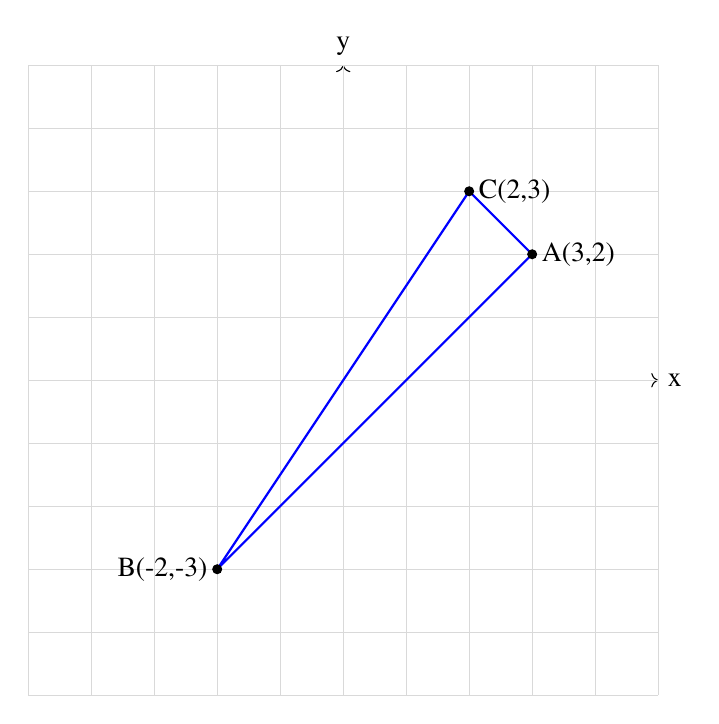
\begin{tikzpicture}[scale=0.8]
    % Draw axes
    \draw[->] (-5,0) -- (5,0) node[right] {x};
    \draw[->] (0,-5) -- (0,5) node[above] {y};

    % Grid (optional)
    \draw[step=1cm,gray!30,very thin] (-5,-5) grid (5,5);

    % Points
    \coordinate (A) at (3,2);
    \coordinate (B) at (-2,-3);
    \coordinate (C) at (2,3);

    % Draw triangle
    \draw[thick, blue] (A) -- (B) -- (C) -- cycle;

    % Draw and label points
    \filldraw[black] (A) circle (2pt) node[anchor=west] {A(3,2)};
    \filldraw[black] (B) circle (2pt) node[anchor=east] {B(-2,-3)};
    \filldraw[black] (C) circle (2pt) node[anchor=west] {C(2,3)};
    \end{tikzpicture}
    
        % Add "Fig. 0" text below the figure
    \vspace{0.5cm} % space between figure and text
    \textbf{Fig. 0}

\end{center}

\end{document}

